\documentclass[notitlepage]{revtex4-2}
% includes...
\usepackage{amsmath}
\usepackage{bm}
\usepackage{natbib}
\usepackage{graphicx}
\usepackage{hyperref}
\usepackage{epstopdf}
\usepackage{color}
\usepackage{tikz}
\usetikzlibrary{arrows.meta}
\tikzset{%
  >={Latex[width=2mm,length=2mm]},
  % Specifications for style of nodes:
            base/.style = {rectangle, rounded corners, draw=black,
                           minimum width=2.5cm, minimum height=1cm,
                           text centered, font=\sffamily},
             box/.style = {base, fill=yellow!60, font=\scriptsize},
            boxs/.style = {base, fill=red!60, font=\tiny},
    activityRuns/.style = {base, fill=green!30},
         process/.style = {base, minimum width=2.5cm, fill=orange!15,
                           font=\ttfamily}

}
\begin{document}
%front matter
\title{VEBISPH code: two dimensional incompressible SPH code for viscoelastic flows}

\author{J. R. C. King}
\email{jack.king@manchester.ac.uk}
\affiliation{Department of Mechanical, Aerospace and Civil Engineering, The University of Manchester, Manchester, M13 9PL, UK}
\date{\today}
\begin{abstract}

A brief description of the VEBISPH code. Numerical methods in this code follow~\cite{king_2021}

\end{abstract}

\maketitle
%end front matter

\section{Directory structure}

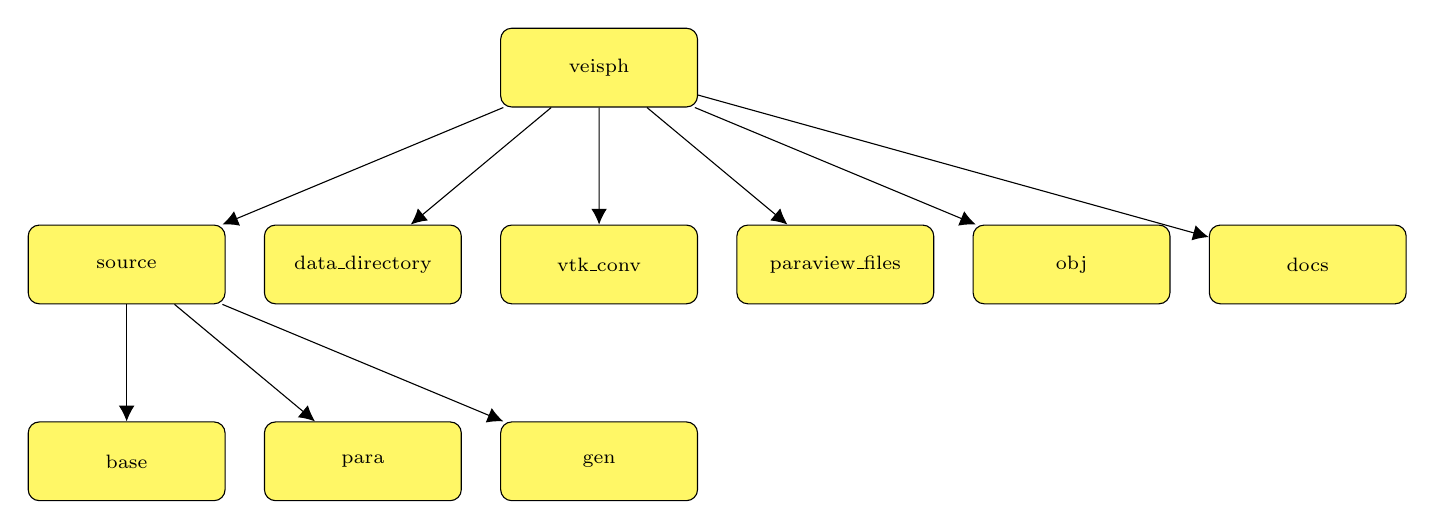
\begin{tikzpicture}[node distance=1.5cm,
    every node/.style={fill=white, font=\sffamily}, align=center]
  % Specification of nodes (position, etc.)
  \node (veisph)       [box, xshift=6cm]                        {veisph};
  \node (source)     [box, below of=veisph, xshift=-6cm, yshift=-1cm]                  {source};
  \node (data)    [box, right of=source, xshift=1.5cm]  {data\_directory};
  \node (vtk)      [box, right of=data, xshift=1.5cm]                {vtk\_conv};
  \node (parav)    [box, right of=vtk, xshift=1.5cm]     {paraview\_files};
  \node (obj)   [box, right of=parav, xshift=1.5cm]  {obj}; 
  \node (docs)   [box, right of=obj, xshift=1.5cm]  {docs};   
  
  \node (base)   [box, below of=source, yshift=-1cm]  {base};
  \node (para)   [box, right of=base, xshift=1.5cm]  {para};
  \node (gen)   [box, right of=para, xshift=1.5cm]  {gen};          

  \draw[->] (veisph) edge (source);
  \draw[->] (veisph) edge (vtk);
  \draw[->] (veisph) edge (parav);
  \draw[->] (veisph) edge (data);
  \draw[->] (veisph) edge (obj);        
  \draw[->] (veisph) edge (docs);          

  \draw[->] (source) edge (base);
  \draw[->] (source) edge (para);
  \draw[->] (source) edge (gen);    
  
  \end{tikzpicture}
  
\begin{itemize}
\item \verb|source| contains source files for the code:
\begin{itemize}
\item \verb|base| contains main modules for VEISPH
\item \verb|para| contains parameters and common variables
\item \verb|gen| contains code to generate casefiles and initial conditions
\end{itemize}
\item \verb|data_directory| contains output files produced by the code
\item \verb|vtk_conv| contains a program to convert output files into \verb|.vtu| files, which can be read by Paraview.
\item \verb|paraview_files| the program in \verb|vtk_conv| creates \verb|.vtu| files here.
\item \verb|obj| contains \verb|.o| and \verb|.mod| files created during compilation.
\item \verb|docs| contains this document...
\end{itemize}  


\section{Governing equations}\label{ge}

The governing equations (here listed in dimensionless form) in the arbitrary frame of reference as in~\cite{king_2021} are:

\begin{subequations}
\begin{align}\nabla\cdot\bm{u}&=0\label{eq:mass}\\
\frac{d\bm{u}}{dt}-\bm{u_{s}}\cdot\nabla\cdot\bm{u}&=-\nabla{p}+\beta\sqrt{\frac{Pr}{Ra}}\nabla^{2}\bm{u}+\frac{\left(1-\beta\right)Pr}{Ra\times{El}}\nabla\cdot\bm{\tau_{p}}+\theta\bm{e_{y}}+\bm{f}\label{eq:mom}\\
\frac{d\bm{A}}{dt}-\bm{u_{s}}\cdot\nabla\bm{A}-\left(\bm{A}\cdot\nabla\bm{u}^{T}+\nabla\bm{u}\cdot\bm{A}\right)&=\frac{-1}{El}\sqrt{\frac{Pr}{Ra}}f_{R}\left(\bm{A}\right)\label{eq:conf}\\
\frac{d\theta}{dt}-\bm{u_{s}}\cdot\nabla\theta&=\frac{1}{\sqrt{Ra\times{Pr}}}\nabla^{2}\theta\label{eq:heat}\end{align}\label{eq:ce}\end{subequations}
where $\bm{u}$ is the velocity, $p$ the pressure, $\theta$ the temperature deviation (from ambient), and $\bm{\tau_{p}}$ is the polymeric stress, related to the conformation tensor $\bm{A}$ by  the strain function 
\begin{equation}\bm{\tau_{p}}=f_{S}\left(\bm{A}\right)=\bm{A}-\bm{I}\end{equation}. The relaxation function $f_{R}$ 
defines the closure of the constitutive model, and in this code is limited to the Linear PTT model with
\begin{equation}f_{R}=\left[1+\varepsilon{tr}\left(\bm{A}-\bm{I}\right)\right]\left(\bm{A}-\bm{I}\right)\end{equation}
where $\varepsilon$ is the degree of non-linearity, and $\bm{I}$ is the identity tensor. When $\varepsilon=0$, the PTT model collapses to the Oldroyd B model. $\bm{f}$ is a body force.

The system is controlled by the four dimensionless quantities:
\begin{subequations}
\begin{align}\beta&=\eta_{s}/\eta_{0}\qquad&\text{Viscosity ratio}\\
Pr&=\frac{c_{p}\eta_{0}}{\kappa}\qquad&\text{Prandtl number}\\
Ra&=\frac{L^{3}\Delta\rho\left\lvert\bm{g}\right\rvert}{\alpha\eta_{0}}\qquad&\text{Rayleigh number}\\
El&=\frac{\lambda\eta_{0}}{L^{2}}\qquad&\text{Elasticity number},
\end{align}\end{subequations}
where $\eta_{s}$ is the solvent viscosity, $\eta_{0}$ is the total viscosity, $c_{p}$ is the specific heat capacity (at const. pressure), $\kappa$ is the thermal diffusivity, $\alpha$ is the thermal conductivity (related to $\kappa$ via density $\rho$ and $c_{p}$), $\bm{g}$ is the acceleration due to gravity, $\Delta\rho$ is a characteristic density deviation, $\lambda$ is the relaxation time and $L$ is a characteristic length-scale.

The Reynolds number is related to these dimensionless groups by: $Re=\sqrt{Ra/Pr}$. The Weissenberg number is $Wi=El\sqrt{Ra/Pr}$.


\section{Numerical implementation}

Full details in~\cite{king_2021}. Spatial discretisation is with SPH operators. Time evolution is with a first-order projection scheme~\cite{chorin_1968}, with divergence free velocity constraint enforced via a Poisson equation, which is solved using a BiCGStab algorithm with Jacobi preconditioner. Boundary conditions are imposed with mirror particles. SPH gradient and divergence operators are corrected to first order following~\cite{bonet_lok}. Temporal evolution of the conformation tensor is via the log-conformation formulation of~\cite{fattal_2004,fattal_2005}, mostly following~\cite{lopez_2019}.

\section{Boundary framework}

The computational domain is described by a set of boundary nodes, connected by straight lines (boundary patches), along with circles. In \texttt{datclass.F90} these are hard-coded for each case. For example, a rectangular domain with solid upper and lower boundaries and periodic lateral boundaries would be defined as:
\begin{verbatim}
     b_type(:) = (/ 1, 2, 1, 2/)
     b_vel(:) = (/ -0.0d0,0.0d0,0.0d0,0.0d0/)    
     b_thermal(:) = (/ 1.0d0,0.0d0,-1.0d0,0.0d0/)
     b_periodic_parent(:) = (/ 3, 4, 1, 2/)
     b_node(1,:) = (/ 0.0d0, 0.0d0 /)
     b_node(2,:) = (/ xl, 0.0d0 /)
     b_node(3,:) = (/ xl, yl /)
     b_node(4,:) = (/ 0.0d0, yl /)
\end{verbatim}
where \texttt{xl} and \texttt{yl} are variables describing the length and height of the domain. The array \verb!b_vel! indicates the velocity (tangential to the boundary patch) and here is usually zero. The array \verb!b_type! indicates whether the patch is a wall ($1$) periodic ($2$), invisible ($0$) or (in other versions, but not relevant to this project) inflow ($3$) or outflow ($4$). For periodic patches, a relationship needs to be defined with a parent patch, which is done via the array \verb!b_periodic_parent!.

Circular obstacles are described similarly, with centre \verb!c_centre!, radius \verb|c_radius|, angular velocity \verb|c_omega| and translational velocity \verb|c_vel|. In this project, the translational velocities will probably always be zero. A positive value of \verb|c_radius| indicates the circle is an internal obstacle (e.g. the inner boundary in Taylor-Couette flow), whilst a negative value indicates the circle is an external boundary (e.g. the outer boundary in Taylor-Couette flow).

\subsection{How boundary conditions are applied in the code}

In the code (\verb|source/base/mirror_boundaries_mod.F90|), the routine runs through all particles and identifies those near boundaries. Then, it runs through each boundary, and for all particles near that boundary, creates a mirror particle in the appropriate place, with appropriate conditions. The code then runs through all corners (i.e. all boundary nodes), and performs a similar procedure. Each mirror particle $j$ has a parent particle $i$, and the array \verb|irelation| tracks this: \verb|irelation(j)=i|. The array \verb|vrelation| stores information (in a confusing way) about the type of boundary which relates a mirror and its parent, and is used in specifying velocity relationships.

For example, if particle $i$ is near a solid boundary patch, a particle $j$ will be created which is a reflection of particle $i$ in the boundary patch. Particle $j$ will have velocity $\bm{u}_{j}=2\bm{u}_{b}-\bm{u}_{i}$, where $\bm{u}_{b}$ is the velocity of the boundary patch.

Pressure boundary conditions ($\bm{n}\cdot\nabla{p}=\bm{f}\cdot\bm{n}$) are constructed by specifying the difference between a mirror and its parent pressure through the array \verb|dp_mp|, such that \verb|P(i) = P(j) + dP_mp(i)|.

\section{Overview of the code structure}

The code consists of modules, each module is stored in a separate \verb|.F90| file. Each module contains one or more subroutines which perform similar tasks, or tasks related to a theme (e.g. the module \verb|part_shift| contains routines related to Fickian shifting).

The main program is contained within \verb|sph2D_incom.F90|. It calls routines from the input module \verb|input.F90|, some other housekeeping, then contains the main time loop. Within the main time loop, the routine \verb|div_free| is called, which performs a single time step, then \verb|output| is called, which saves any data as required. The module \verb|div_free.F90| is the heart of the code, and is fairly clearly commented, the the subroutine \verb|divfree| corresponds (roughly) to the steps $1$ to $7$ on pages 5 and 6 of~\cite{king_2021}.

\section{Case creation, compiling, running and postprocessing}

\subsection{Case creation}\label{case}

In the directory \texttt{source/gen/} there is a file \texttt{datclass.F90}. This is the main part of a program which generates the input data for the code. Navigate to this directory, and then build and run it with:
\begin{verbatim}
make
./gen2D
cp I* ../../.
\end{verbatim}
When you run \verb|./gen2D|, it will give a list of cases and prompt you to choose one. Type the relevant number and press enter. You can modify \verb|datclass.F90| to create more cases.

The following cases are currently included in \verb|datclass.F90|:
\begin{enumerate}
\item 2D dam break
\item Taylor Green vortices
\item Poiseuille flow
\item Rayleigh-Benard flow
\item Periodic cylinders in a channel (as in~\cite{vazquez_2012})
\item Free-surface Rayleigh-Benard.
\item Plane Couette flow
\end{enumerate}

\subsection{Compiling and running the code}

The Makefile is built for systems with the compiler \verb|gfortran| install. If using an alternative compiler, modify the lines \verb|FC := gfortran| and \verb|LD := gfortran| to point to your chosen compiler. You need a system with OpenMP installed.

To compile and run the code,
\begin{enumerate}
\item Navigate the main directory \verb|vebisph|
\item Compile the code with the command \verb|make const_mod=X|, where $X=1$ will compile for Newtonian flows, and $X=2$ will compile for viscoelastic flows.
\item Run the code by typing \verb|./vebisph|
\end{enumerate}

\section{Post-processing}

Data from the code are saved in the folder \verb|data_directory|. Within the folder \verb|vtk_conv| there is a small program which converts the data into a format which can be read by Paraview. 

To process the results
\begin{enumerate}
\item Navigate in a terminal to \verb|vtk_conv|
\item Run \verb|./a.out| (you may need to recompile it, with \verb|gfortran PART2VTU_2D.f| first.
\item The files which paraview can read will be created in the folder \verb|paraview_files|
\end{enumerate}

To view the files, open paraview, and open the files \verb|PART00XX|.

Additional outputs/diagnostics are saved as files called \verb|fort.XXX|. For example, a routine in \verb|div_free.F90| writes the maximum velocity in the domain at each output time to the file \verb|fort.192|.

\section{Linux tips}
\begin{itemize}
\item Use tab key to autocomplete commands;
\item \verb|cd ../| navigates up one level;
\item Similarly, \verb|cp x ../.| copies file \verb|x| up one level;
\item Use up/down arrow keys to scroll through command line history;
\item Ctrl+shift+N opens a new terminal;
\item In a file browser, you right click $\to$ open in terminal;
\item Ctrl+C aborts a program.
\end{itemize}


\bibliographystyle{elsarticle-num-names}
\bibliography{jrckbib}

\end{document}


